\section{Synthesising OSPF Configurations} \label{sec:synthesis}
In this section, we present an algorithm for 
solving the path-compliance problem for networks
with a single domain---i.e., $|\{\Theta(n) \mid n\in V\}|=1$.

%\subsection{Complexity} \label{sec:rfcomplexity}

Before we present our technique and its intricacies,
we justify the complexity of our approach by showing that
the problem of synthesizing an OSPF configuration
that contains an optimal number of rout filters is NP-complete.

\begin{theorem}
Given a set of paths $\Pi$,
a topology $G=(V,E)$,
a domain-assignment function $\Theta$, such that $|\{\Theta(n) \mid n\in V\}|=1$,
a number $n\geq 0$,
the problem of finding 
an $LP$, $W$, and $RF$,  such that
\loris{PC shouldn't appear here, make consistent.}
$\paths(\Theta, LP, W, RF, PC) = \Pi$,
and 
$\sum_{\lambda\in\Lambda} |RF(\lambda)|=n$, is NP-complete.
\end{theorem}
\iffull
%!TEX root = paper.tex
\begin{proof}
We show that the decision version of the minimum 
vertex cover problem, i.e., there exists a vertex cover
of size $ \leq k$, which is NP-complete, 
reduces to finding a set of static routes 
of size $ \leq k$ \
and OSPF weights for a network with only one domain. 
The latter is also in NP, so after the reduction we 
can conclude that it is also NP-complete.

Let $G = (V,E)$ be an instance of the 
minimum vertex cover problem. A set of
vertices $VC \subseteq V$ is the vertex cover
if $\forall (v_1, v_2) \in E. ~v_1 \in VC \vee v_2 \in VC$. 

We now show how to construct a topology $T=(S,L)$ 
and a corresponding set of paths $\Pi$ that can be enforced 
by configuration C which requires static routes $SR$ such that $|SR| \leq k$  
if and only if the corresponding $VC(SR)$ is a vertex cover of 
the graph $G$ and $|VC(SR)| \leq k$.

\paragraph{Construction.}
For every vertex $v \in V$: add a vertex $r_v$.
For every edge $(u,v) \in E$: add two vertices $s_{uv}$
and $t_{uv}$ to $S$. Add edges
connecting $s_{uv} \rightarrow r_{u}$, $s_{uv} \rightarrow r_{v}$,
$r_{u} \rightarrow t_{uv}$ and $r_{v} \rightarrow t_{uv}$. 
\Cref{fig:rfcomplexity} illustrates this construction.
\begin{figure}[H]
	\centering
	\begin{tikzpicture}[shorten >=0.5pt,node distance=1.5cm,on grid,auto,
	square/.style={regular polygon,regular polygon sides=4}] 
	\node[state] at (0,0) (s)  {$s_{uv}$}; 
	\node[state] at (3,-1) (v)  {$r_v$}; 
	\node[state] at (3,1) (u)  {$r_u$}; 
	\node[state] at (6,0) (t) {$t_{uv}$}; 	
	\node[state] (s1) [below=of s] {$s_{vw}$}; 	
	\node[state] (t1) [below=of t] {$t_{vw}$}; 	
	\path[-] 
	(s) edge  node {} (v)
	edge  node {} (u)
	edge [blue, dashed, bend right=40] node {} (t)
	edge [red, dashed, bend left=40] node {} (t)
	(u) edge node {} (t)
	(v) edge node {} (t)
	edge node {} (t1)
	edge node {} (s1);
	\path[->]
	(s)
	edge [blue, dashed, bend right=40] node {} (t)
	edge [red, dashed, bend left=40] node {} (t);
%	\path[-] (s) edge node[above] {} +(1,-0.1);
%	\path[-] (t1) edge node[above] {} +(-1,-0.1);
	\end{tikzpicture}
	\caption{Construction for reduction to Vertex Cover.}
	\label{fig:rfcomplexity}
\end{figure}
If there is another edge $(v,w) \in E$, then
$s_{vw}$ and $t_{vw}$ have an edge connecting to $r_v$ (shown
in \Cref{fig:rfcomplexity}). 

For each edge $(u,v) \in E$, we add two paths in $\Pi$: 
$s_{uv} \rightarrow r_u \rightarrow t_{uv}$
for destination host $d_u$ and 
$~s_{uv} \rightarrow r_v \rightarrow t_{uv}$ 
for destination host $d_v$.
(dashed paths in \Cref{fig:rfcomplexity}). 

We now prove that if there exists a set of static routes
$SR$ such that $|SR| \leq k$ such that the resulting configurations
are path-compliant for $\Pi$, then there exists a vertex cover $VC$
of $G$ such that $|VC| \leq k$. 

For each static route $sr \in SR$, the static route
has to be placed at the source, either going to $r_u$
or $r_v$ (structure of topology $T$). 
We construct a set $VC(SR)$ by adding the vertex $v$
based on the endpoints of each static route $sr \in SR$.
To show that $VC(SR)$ is a vertex cover of $G$, we first
prove \Cref{lemma:diamond}.

\begin{lemma} \label{lemma:diamond}
	 For each diamond formed by the input paths, atleast 1 
	 static route on one of the edges of the paths of the diamond 
	 is required to find a valid solution to the
	 OSPF edge weights.  
\end{lemma}

\begin{proof}
Given two paths $\pi_1$ and $\pi_2$ for destinations 
$d_u$ and $d_v$, we define these paths form a diamond
if these paths intersect at two routers ($s_{uv}$ and $t_{uv}$) 
without any common router in between. 
Consider the following diamond % in \Cref{fig:diamond}
constructed by paths $\pi_1$: $s_{uv} \rightarrow r_u \rightarrow t_{uv}$ 
for destination $d_u$ and $\pi_2$: $s_{uv} \rightarrow r_v \rightarrow t_{uv}$ 
for destination $d_v$. Let us assume there exists a solution 
for the OSPF edge weights without any static routes. 

We add the following inequality 
to make $\pi_1$ is the shortest 
path from $s_{uv}$ to $t_{uv}$ by
ensuring
 $\pi_1$ is shorter than the
path from $s_{uv}$ to $t_{uv}$ via $r_v$: 
\begin{equation} \label{eq:diamond1}
	W(s_{uv},r_u) + W(r_u, t_{uv}) < W(s_{uv}, r_v) + W(r_v,t_{uv})
\end{equation}
Since $\pi_2$ is also the shortest path from $s_{uv}$ 
to $t_{uv}$, the linear inequality added is:
\begin{equation}  \label{eq:diamond2}
W(s_{uv},r_v) + W(r_v, t) < W(s_{uv}, r_u) + W(r_u,t_{uv})
\end{equation}
Since there are no static routes on the edges
of $\pi_1$ and $\pi_2$, none of the above equations are 
eliminated. 
Adding equations \ref{eq:diamond1} and  \ref{eq:diamond2} 
yields the inequality $0 < 0$, which is inconsistent 
and therefore, no solution to 
the edge weights exists for this system of equations, 
which contradicts our assumption. Therefore,
for each diamond formed by the input paths, atleast 1 
static route on one of the edges of the paths of the diamond 
is required to find a valid solution to the
OSPF edge weights.  
\end{proof}

For every edge $(u,v) \in E$, the constructed paths from 
$s_{uv}$ to $t_{uv}$ form a diamond. Thus, by Lemma~\ref{lemma:diamond}, 
the diamond created by the paths corresponding to each edge in $G$ 
requires atleast one static route to eliminate
the inconsistency caused by the diamond. If a static route's endpoints
contains $r_u$, we put $u$ in $VC(SR)$ and similarily for $r_v$. 
Edge $(u,v)$ is covered since atleast one static route is added,
thus, atleast one of $\{u,v\}$ is in $VC(SR)$.  
Thus, if $SR$ eliminates all diamond inconsistencies
to find a solution to the OSPF weights, the corresponding set
$VC(SR)$ covers all edges in $E$. Therefore, $VC(SR)$ is a vertex
cover. 

Thus, by finding a set of static routes $SR$ such that $|SR| \leq k$
such that all the diamond inconsistencies are eliminated, and there
exists OSPF weights $W$ such that the configurations forward traffic
along $\Pi$, we can find a vertex cover $VC$ for graph $G$ such that
$|VC| \leq k$. 

This transformation is polynomial, the constructed 
network topology $T$ has $|V| + 2|E|$ nodes, 
$4|E|$ links and $2|E|$ paths. Therefore, OSPF
configuration synthesis with number of static routes $\leq k$ is
NP-complete. Thus, OSPF synthesis with minimal number of 
static routes is NP-hard. 
\end{proof}

\fi


\subsection{From paths to ARCs} \label{sec:phase2}

The second phase of our approach takes as input the set of paths produced by the first phase
and produces an Abstract Representation of the Control Plane (ARC) that realizes the given set of paths.
First, we consider the problem of generating ARCs that
 forward packets based on shortest-paths---e.g., OSPF routing.
Then, we consider more complex forms of ARCs in which 
 additional mechanisms like route-filtering are allowed. 
 
\subsubsection{From paths to simplified ARCs} \label{sec:sarc}
The \emph{Simplified Abstract Representation of the Control Plane} (sARC) is a directed graph comprising ritches as 
vertices and weighted edges corresponding to all links in the
topology. 
This is an ideal control plane supporting classic shortest path routing in which no links can be disabled. 

The problem of synthesizing 
a sARC that realizes an input set of paths reduces to a
variation of the so-called {\em inverse shortest path} problem~\cite{isp}. 
Assume we are given the following inputs: (1) a directed graph $T = (S, L)$ (the network topology), 
(2) a set of endpoints $\Gamma \subseteq S\times S$
describing the sources and destinations of the input paths, and 
(3) a function $P: \Gamma \rightarrow 2^{L^*}$
that assigns to each pair of endpoints $(s,t) \in \Gamma$ 
a set of \emph{acyclic} paths, such that for every path $l_0\cdots l_n\in P(s,t)$,
$l_0=(s,s')$, for some $s'\in S$, and $l_n=(s'',t)$, for some $s''\in S$.\footnote{
We use $L^*$ the denote the set of all finite sequences over $L$.}
The 
\emph{sARC synthesis}
problem is to find rational weights for the edges in $L$ such that 
for each pair of endpoints $(s,t) \in \Gamma$, 
the paths in $P(s,t)$ are \emph{the} shortest paths from $s$ to $t$ 
in the graph. Notice, that there can be multiple shortest
paths of equal cost for multi-path support (e.g., for traffic engineering).

In sARC, packet forwarding is based on destination.
For a destination $d$, we call $\xi_d$ the directed
subgraph of $T$ obtained by only keeping the nodes and edges 
that are traversed by paths with destination $d$.
Since paths are acyclic, $\xi_d$ is a directed acyclic graph.
We use $\Omega=\{d\mid (\_,d)\in\Gamma\}$ to denote the 
set of all destinations and $\Delta=\{\xi_d\mid d\in \Omega\}$ to denote  
the set of all destination DAGs. 

We use  $r_1\rightarrow r_2$ to denote $(r_1,r_2)\in L$ and
$r_1\rightarrow^* r_2$ (resp. $r_1\rightarrow^+ r_2$) to denote 
that $r_2$ is reachable from $r_1$ by crossing zero (resp. one) or more links in $T$.
Similarly, we use $\rightarrow_{\xi_d}$ to denote the same relations in the destination DAGs.


\minisection{Distance equations}
To solve the sARC synthesis problem, we generate a set of linear equations
to find the required edge weights. 
We use $E(r_1, r_2)$ to denote the weight of the edge $(r_1,r_2)\in L$
and 
$D(r_1, r_2)$ to denote the shortest distance from $r_1$ to $r_2$.
We add the equation $D(s,s) = 0$ for every $s\in S$ to denote that the distance
from a node to itself is $0$.
The
following equation guarantees that $D(s,t)$ is not greater than 
the actual shortest distance from $s$ to $t$.
\begin{multline} \label{eq:dist}
\forall s, t, r. (s \rightarrow r \rightarrow^* t).\\
D(s, t) \leq E(s, r) + D(r, t)
\end{multline}

For each destination DAG $\xi_d\in\Delta$, we add equations to ensure 
that the input paths with destination $d$ are indeed the shortest ones.
 If a path
is the shortest path between its endpoints, then every 
subpath of the path has to be the shortest between its endpoints
as well (otherwise the complete path would not be the shortest).

% \begin{figure}[h!] 
% 	\centering
% 	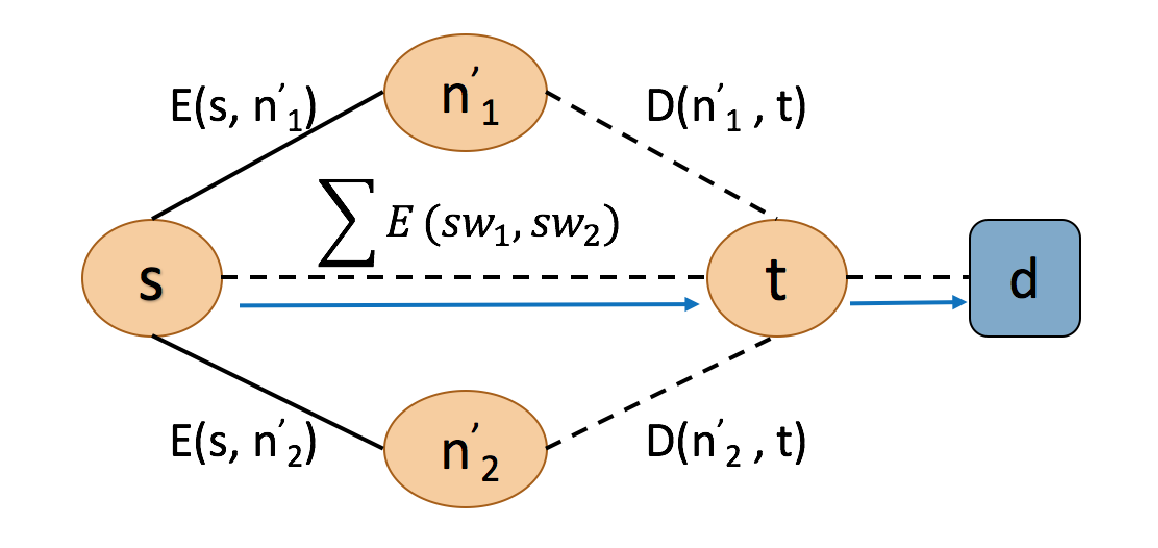
\includegraphics[width=0.75\columnwidth]{figures/distanceEquation.eps}
% 	\caption{An example illustration of the distance equations for shortest path forwarding.
% 		The pointed arrows represent the path in DAG of destination $d$, and the
% 		dotted line represents 1 or more edges. 
% 	} \label{fig:disteq}
% \end{figure}
Consider a DAG $\xi_d$ for destination $d$. We define two neighbour
functions: $N_T(s)$ denotes the set of neighbours of ritch $s$ 
in the input graph $T$, and $N_{\xi_d}(s)$ denote the set of
neighbours of ritch $s$ in the destination DAG $\xi_d$. 
Given a destination $d\in \Omega$,
we use the following equations to ensure that, given two nodes $s$ and $t$ in
$\xi_d$, 
the set of paths from $s$ to $t$ in $\xi_d$ are
exactly
\emph{the} shortest paths from $s$ to $t$ in $T$.
Let $s$ and $t$ be two nodes in $\xi_d$ and let  $Paths_{\xi_d}(s,t)$ be the set of paths from $s$ to $t$ in $\xi_d$.
\begin{multline} \label{eq:uniq1}
		\forall l_0\cdots l_n\in Paths_{\xi_d}(s,t).
		\forall n' \in N(s) \setminus N_{\xi_d}(s). \\
		E(s, n') + D(n', t) > \sum_{\mathclap{\substack{l_i=(s_i,t_i)}}} 
		E(s_i, t_i) 
\end{multline}
\begin{multline} \label{eq:uniq2}
		\forall l_0\cdots l_n\in Paths_{\xi_d}(s,t).
		\forall n' \in N_{\xi_d}(s). n' \not\rightarrow^+_{\xi_d} t.  \\
		E(s, n') + D(n', t) > \sum_{\mathclap{\substack{l_i=(s_i,t_i)}}} 
		E(s_i, t_i) 
\end{multline}
\vspace{-2mm}
\begin{multline} \label{eq:uniq3}
		\forall l_0\cdots l_n, l_0'\cdots l_n'\in Paths_{\xi_d}(s,t).\\
		\sum_{\mathclap{\substack{l_i=(s_i,t_i)}}} 
		E(s_i, t_i)  =\sum_{\mathclap{\substack{l_i'=(s_i',t_i')}}} 
		E(s_i', t_i') 
\end{multline}
Equation~\ref{eq:uniq1} guarantees that 
the sum of the weights belonging to a path from $s$ to $t$ in $\xi_d$ is smaller than 
any path that goes to $t$ via a node $n'$ that is a neighbour of $s$ in $T$ but not in $\xi_d$.
Equation~\ref{eq:uniq2} guarantees that
the sum of the weights belonging to a path from $s$ to $t$ in $\xi_d$ is smaller than 
any path that goes to $t$ via a node $n'$ that is a neighbour of $s$ in $\xi_d$ but such that
$t$ is not reachable from $n'$ in $\xi_d$.
Finally, Equation~\ref{eq:uniq3} guarantees that all the paths from $s$ to $t$ in $\xi_d$ have the same weight.
